%!TEX root=./report.tex
\section{Empirical study}
In this section we discuss the experimental results using the proposed measures and their implications on different phenomena seen in practice regarding the generalization behavior.

\subsection{Difference between true and random labeled data}
\begin{figure}
	\centering
	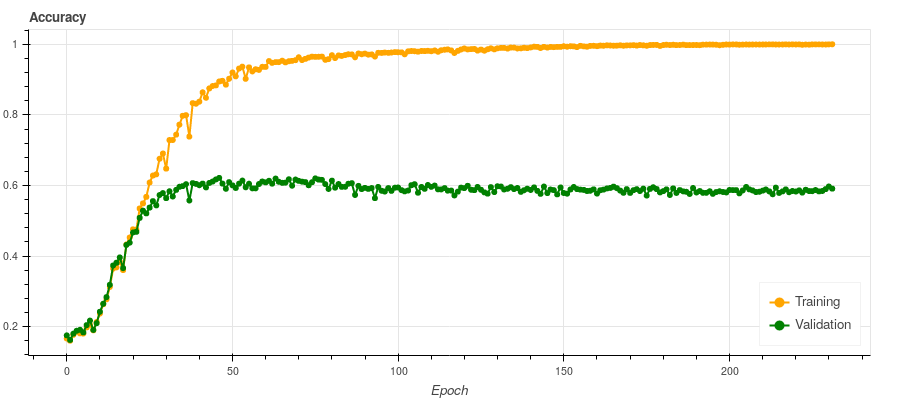
\includegraphics[width=0.24\linewidth]{vgg16/bokeh_plot.png}
	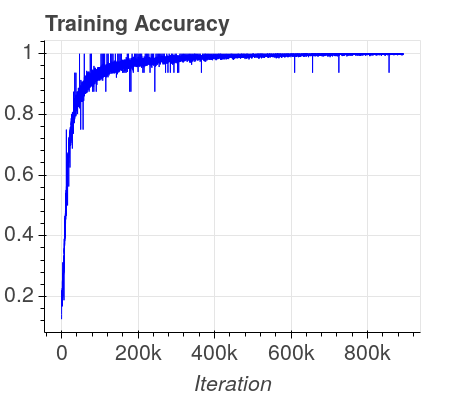
\includegraphics[width=0.24\linewidth]{vgg16/bokeh_plot(1).png}
	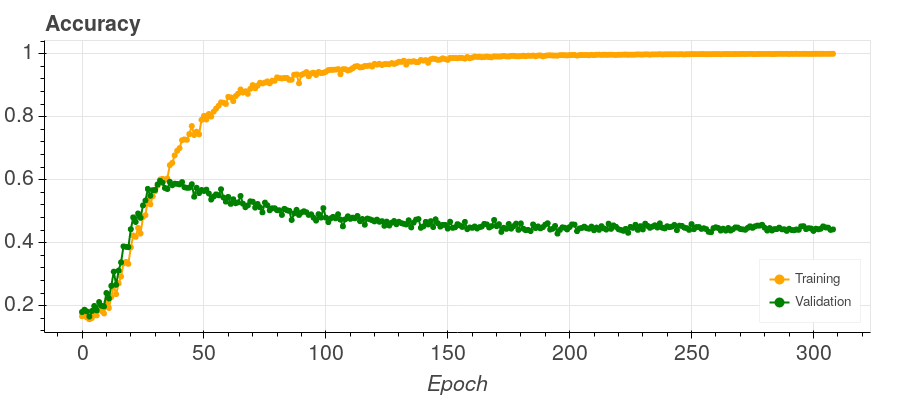
\includegraphics[width=0.24\linewidth]{vgg16/bokeh_plot(2).png}
	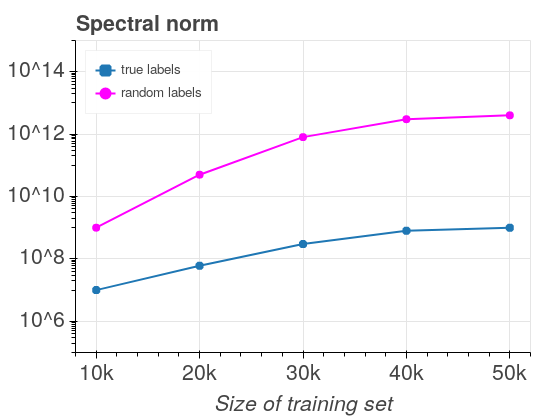
\includegraphics[width=0.24\linewidth]{vgg16/bokeh_plot(3).png}
	\caption{The proposed norms calculated on the network weights of the VGG model \cite{simonyan2014deep} after training on random (magenta) and true (blue) labeled subsets of CIFAR-10 are displayed. We see only a small increase of the measures on true labels but a huge increase using random labels and the measures on random labels to be bigger for every subset. }	
	\label{fig:norms-paper}
\end{figure}
It is possible to obtain zero training error on random labels using the same architecture for which training with real labels leads to good generalization. We would expect the networks learned using real labels (and which generalizes well) to have much lower complexity, under the suggested measure, than those learned using random labels (and which obviously do not generalize well). \cite{neyshabur2017exploring} \par
%
\freff{fig:norms-paper} shows the results of \cite{neyshabur2017exploring}. We see that training the network on true labels (blue) only results in small increases of the norm-based capacity measures in comparison to the increases when training on random labels (magenta). As the network learns the true functional dependence between the input and output using true labels it only requires small increases in complexity as the subset size increases, whereas it requires more capacity for every newly seen data point when using random labels as it needs to memorize the data point.\\
We also see that the norm-based capacity measures are all bigger for random labeled data as the network has to memorize the data whereas the dependence between the input and output can be learned with lower capacity on true labeled data.
%
\subsubsection{Problems reproducing results}
\begin{figure}
	\centering
	\includegraphics[width=0.45\linewidth]{cifar10}
	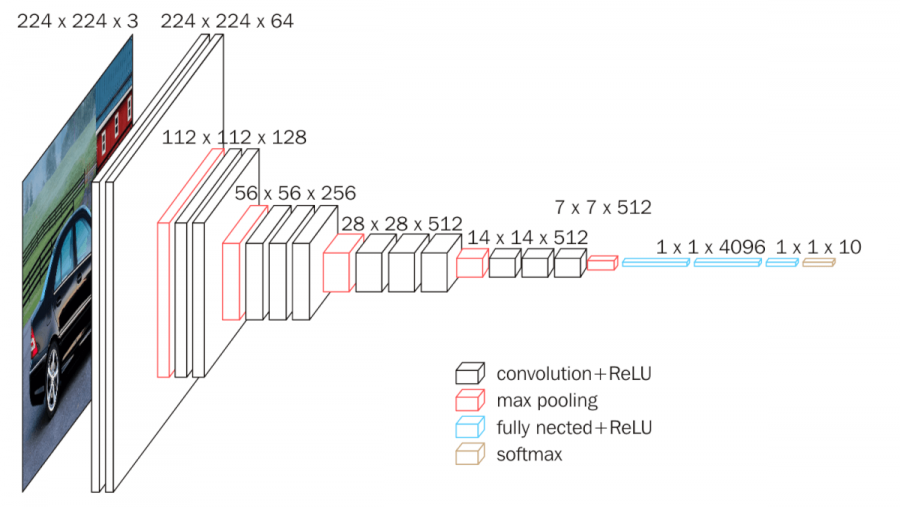
\includegraphics[width=0.45\linewidth]{vgg16}
	\caption{Left: A subset of the CIFAR-10 small image data set with ten classes. Right: The used implementation of the VGG-16 network with batch normalization.}	
	\label{fig:cifar-vgg}
\end{figure}
\begin{figure}
	\centering
%	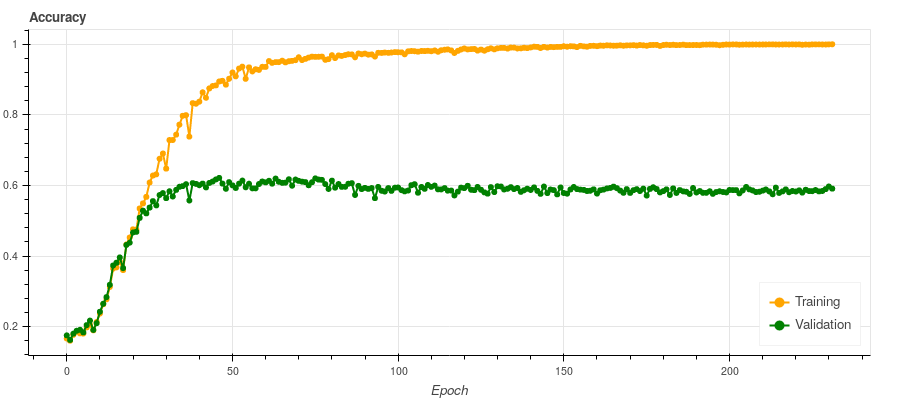
\includegraphics[width=0.24\linewidth]{vgg16/bokeh_plot.png}
	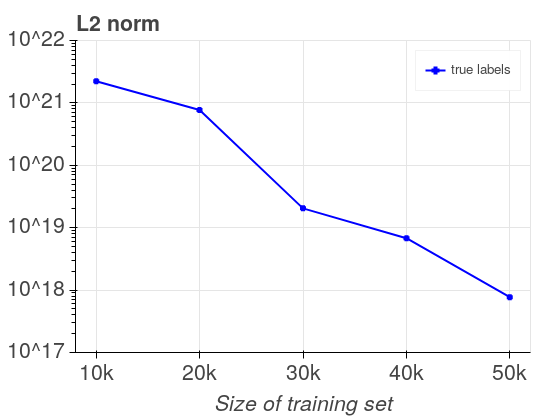
\includegraphics[width=0.24\linewidth]{vgg16/l2_own.png}
%	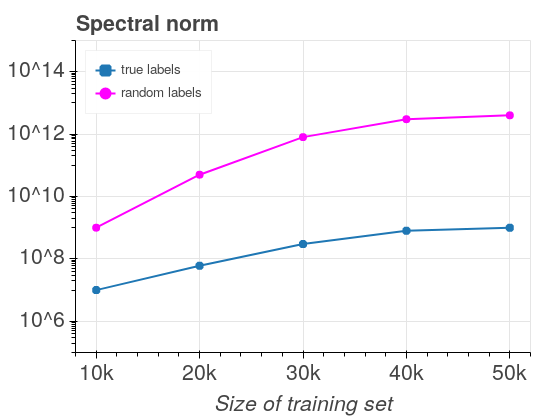
\includegraphics[width=0.24\linewidth]{vgg16/bokeh_plot(3).png}
	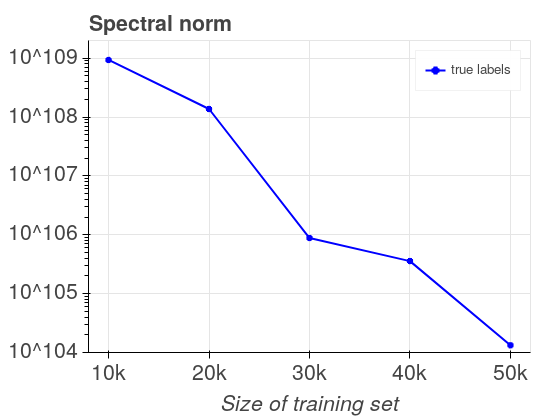
\includegraphics[width=0.24\linewidth]{vgg16/spectral_own.png}
	\caption{The $l2$ and spectral norm calculated on the network weights of the VGG-16 model after training on subsets of CIFAR-10 are displayed. The results show no reproducibility of the results presented by \cite{neyshabur2017exploring}.}	
	\label{fig:norms-own}
\end{figure}
Following the vague instructions of \cite{neyshabur2017exploring} the VGG-16 network with batch normalization \fref{fig:cifar-vgg} is trained on different subsets of the CIFAR-10 \fref{fig:cifar-vgg} data set. For every subset a copy with the labels replaced by random labels has been created and the model is trained on both the true and random labeled subset. \\
%
The huge scope for interpretation of the approach used in \cite{neyshabur2017exploring} caused the non reproducibility of the results. The problems we face are:
%
\paragraph{Reproduction of network training}
\ns{} only stated that their results were produced using VGG. As VGG is a class of CNN architectures with varying depths and optional batch normalization a grid search over the implementations is performed. Considering the capacity vs. training time trade-of the best results were achieved using VGG-16 with batch normalization.\\
Furthermore, \cite{neyshabur2017exploring} didn't provide information on the used solving strategy. Therefore, we tried simple stochastic gradient descent and Adam but stuck with the later as of the faster convergence.
%
\paragraph{Calculation of norms}
The calculation of path norms is trivial for the fully connected case but not for convolutional layers. As we need to enumerate every path through the network we need a way to associate the layer neurons of succeeding layers when applying a convolution. In the short time of this paper we couldn't come up with a feasible implementation which made it impossible to reproduce the path norms.
%
\paragraph{Training on random labeled data}
Following the missing details of the network implementation and solving strategy a training on random labeled data was not possible. The network didn't overcome a $1/10$ test accuracy on random labels which represents a random choice of the result by the network out of the $10$ classes in the CIFAR-10 data set.

\paragraph{Training time}
The short scope of the seminar enclosing this paper combined with training times ranging from roughly five hours on the smallest subset ranging up to over one day for the biggest one resulted in only small search intervals for the grid search used on the hyperparameters as well the different algorithmic and architectural choices.
%
\subsection{Difference between local minima}
When training the same architecture, with the same training set, using two different optimization methods (or different algorithmic or parameter choices), one method results
in better generalization even though both lead to zero training error. We would
expect to see a correlation between the complexity measure and generalization ability among
zero-training error models. \cite{neyshabur2017exploring}

\subsection{Implications of different hidden unit sizes}
Increasing the number of hidden units, thereby increasing the number of parameters, can
lead to a decrease in generalization error even when the training error does not decrease.
We would expect to see the complexity measure decrease as we increase the number of
hidden units. \cite{neyshabur2017exploring} 